\chapter{Fundamentals of Electron Spin Resonance Spectroscopy}
\label{ch:epr}

In this chapter, the phenomenon of electron paramagnetic resonance is briefly described with details that are required to interpret the spectra of a charging electrochemical cell containing nitroxide radicals attached to a conjugated polymer backbone. After the introduction of the spin Hamiltonian, an experimental procedure to observe the corresponding spin transitions with continuous microwaves is described. The characteristic spectra of nitroxide radicals in various environments are described. Finally, the fundamentals and the experimental techniques of the pulsed EPR spectroscopy are introduced.

\section{The Spin Hamiltonian}
\label{sec:spin}
\paragraph*{Electron Spin}
In the Poincaré group of special relativity~\cite{poincare_1905}, rotations are considered together with the relativistic boosts~\cite{einstein_s_rel} and there emerges an additional quantity that is associated with rotation and is preserved together with the orbital angular momentum. This additional quantity is an integral of motion for point objects rotating around themselves. It is called spin~\cite{kuprov_2023}. A particle is said to have a spin if the quantum mechanical states of the particle in its own rest frame are eigenstates of the square of the angular momentum operator~\cite{Tung_book}. Spin is quantized~\cite{SternGerlach1922}; it can take values in integer- or half-integer multiples of the Planck's quantum of action $\hbar$ up to a certain magnitude $S$. The electron, as a fundamental particle and a fermion, bears a half-integer spin with a magnitude of $S=1/2$~\cite{SternGerlach1922,Sakurai}. 

\par
An isolated electron has two degenerate spin states - spin-up $\vert{\uparrow}\rangle$ and spin-down $\vert{\downarrow}\rangle$ - that are eigenfunctions of the square of the spin operator $\hat{s}^2$ with the same (degenerate) eigenvalue: 
\begin{equation}
\hat{s}^2\vert{\uparrow}\rangle=\frac{3}{4}\hbar^2\vert{\uparrow}\rangle\,\,\,\,\,\,\,\,\,\,\,\,\,\,\
\hat{s}^2\vert{\downarrow}\rangle=\frac{3}{4}\hbar^2\vert{\downarrow}\rangle
\end{equation}
The states $\vert{\uparrow}\rangle$ and $\vert{\downarrow}\rangle$ are also eigenfunctions of the $z$ component of the spin operator, but correspond to different (non-degenerate) eigenvalues $m_s=\pm\hbar/2$~\cite{Sakurai}: 

\begin{equation}
\label{eq:sz_states}
\hat{s}_Z\vert{\uparrow}\rangle = +\frac{\hbar}{2}\vert{\uparrow\rangle}\,\,\,\,\,\,\,\,\,\,\,\,\,\,\hat{s}_Z\vert{\downarrow\rangle}=-\frac{\hbar}{2}\vert{\downarrow\rangle}
\end{equation}


\paragraph*{$\textbf{g}$ factor}

Spin combines with the charge of the electron to endow the electron with a magnetic moment $\mu_{spin} = \gamma S$, where $\gamma=\frac{g_e\mu_B}{\hbar}\approx 28$~GHz/T is the gyromagnetic ratio of the electron, $\mu_B=\hbar e/m_e$ is the Bohr magneton and $g_e \approx 2$ is the electron $g$ factor~\cite{Carrington_g_factor}. The $g$ factor connects the spin of a particle with a magnetic moment that the particle expresses through interactions with external fields~\cite{Schwinger1948}. The Dirac quantum theory of the electron predicts $g_e=2$~\cite{dirac1928}. However, up to date, $g_e=-2.00231930436118(27)$ has been measured to the unprecedented accuracy of 0.13~ppt~\cite{Fan2023_PRL}. This 2022 measurement lies at the frontier of modern particle physics and the accordance of the measured $g_e$ with the value obtained with quantum electrodynamics~\cite{Schwinger1948,Fan2023_PRL} is the triumph of the quantum field theory~\cite{Feynman_1949}. 
\par
Depending on the local environment of an electron, its observed $g$ factor can deviate from $g_e$ due to the spin-orbit coupling that changes the observed magnetic moment of the electron~\cite{Carrington_g_factor}. The magnetic moment of an electron can therefore be used as an extremely sensitive probe of the electron's local environment. The $g$ factor of an electron localized in a molecular orbital can be anisotropic, depending on the shape of the orbital. Anisotropic $g$ factor is represented by a $3\times3$ $\textbf{g}$ matrix that can almost always be diagonalized~\cite{Carrington_g_factor} by an appropriate rotation of the molecular coordinate system.

\paragraph*{The Spin Hamiltonian}
For the interactions considered in this thesis, the following Hamiltonian will be applied to describe the interactions of unpaired electron spins with their local environments, ranging by their magnitude:
\begin{equation}
\label{spin_hamiltonian}
H = H_{EZ} + H_{NZ} + H_{J} + H_{HF} + H_{NQ}
\end{equation}

The electron Zeeman term $H_{EZ}$ defines the largest energy splitting observed in an EPR experiment. It sets the requirements on the hardware and determines the range of the applied magnetic fields. The electron Zeeman splitting reveals the electron's $\textbf{g}$ matrix. If the electron situates next to an $I>0$ nucleus, its local magnetic field has offsets, depending on the orientation of the nuclear spin with respect to the external magnetic field. Those offsets or splittings are described by the nuclear Zeeman term $H_{NZ}$. The hyperfine interaction term $H_{HF}$ describes the hyperfine interaction of the electron spin to the spins of its neighboring nuclei. The measurement of $H_{HF}$ allows for a reconstruction of the hyperfine coupling tensor. The hyperfine coupling tensor and the $\textbf{g}$ matrix can be used as fingerprints to identify the molecular structure and dynamics of the mobile molecular fragments that are released during the operation of an electrochemical cell. The exchange interaction term $H_{J}$ defines the energy that neighboring electron spins need to have in order to exchange their orbitals. $H_{J}$ scales with the concentration of the electrons, and it is used to characterize the packing of the molecular fragments in the electrode. The nuclear quadrupole interaction term $H_{NQ}$ describes the interaction of the nuclear quadrupole moment to the gradient of the electric field at the nuclear coordinates. The nuclear quadrupole moment appears in nuclei with $I>1/2$ due to an asymmetric distribution of the positive charge within the nucleus~\cite{Schweiger2001}. $H_{NQ}$ may lead to noticeable spectral distortions in a highly charged nitrogen-containing $(I=1)$ cathode film, where electric field gradients caused by unevenly charged microscopic domains may be comparable to the electric field gradient caused by the asymmetric electronic orbitals of nitrogen. The terms of Eq.~\ref{spin_hamiltonian} are considered in details in the following five paragraphs.

\begin{figure}[h]
\center
	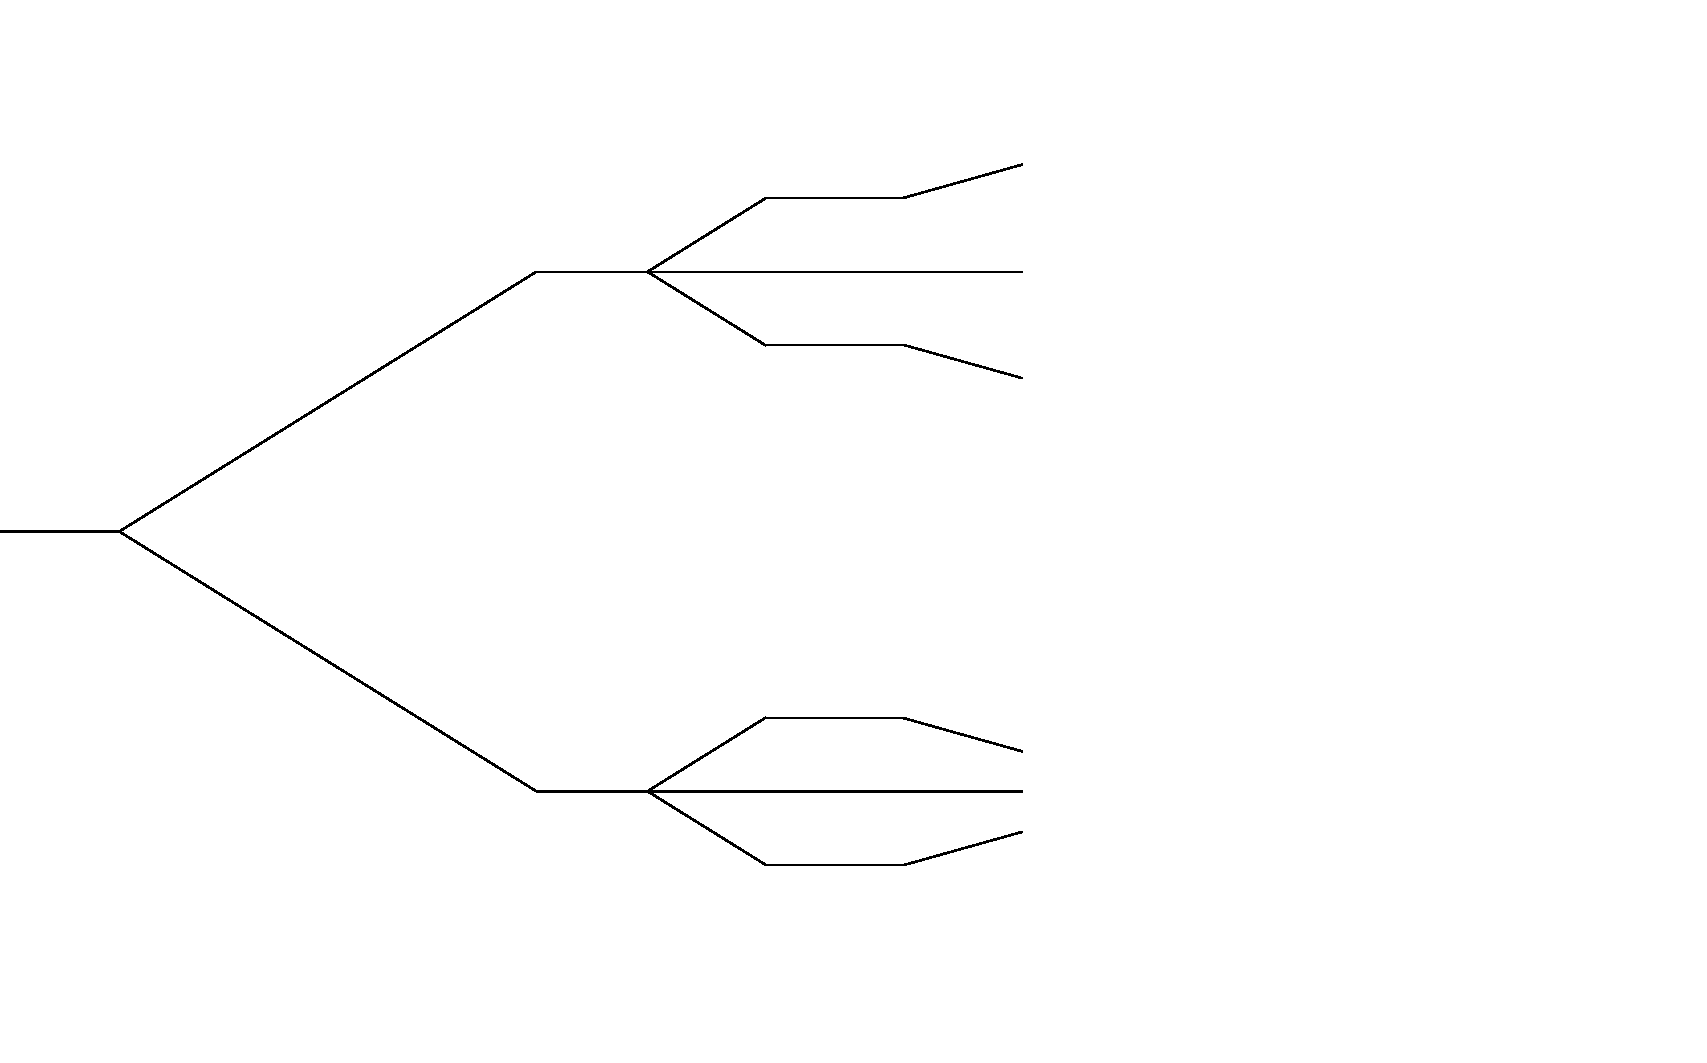
\includegraphics[width=1.0\textwidth]{./operando_epr/figures/energy_diagram.pdf}
	\caption{Energy diagram of the spin Hamiltonian showing the contributions to the energy level of an unpaired electron in a molecular orbital in the presence of Nitrogen. The energy of the unpaired electron at the molecular orbital (MO) splits into two electron Zeeman spin levels $\vert{\uparrow\rangle}$ and $\vert{\downarrow\rangle}$ in the magnetic field. The electron Zeeman spin levels further split into three nuclear Zeeman sublevels, due to the nuclear Zeeman interaction of the Nitrogen nucleus with three projections of the nuclear spin ($m_I=-1,0,+1$). The hyperfine interaction between the electron spin and the nuclear spin depend on the relative orientations of the spins of the particles. The parallel alignment adds $a_{iso}m_Im_s = a_{iso}/2$ to the energy level and the anti-parallel alignment subtracts $a_{iso}m_I(-1)m_s = -a_{iso}/2$ from it. The energy scale for a typical X-band EPR spectrometer is shown on the right. The allowed electron spin transitions corresponding to $\Delta m_s=\pm 1$, $\Delta m_I=0$ are shown in red vertical lines on the right.}
	\label{fig:energy_diagram}
\end{figure}


\paragraph*{Zeeman Splitting}

When an electron is placed in a static magnetic field $\vec{B_0}=B_0 \vec{e_z}$, its magnetic moment experiences a torque and precesses in the $xy$ plane about the field axis with the Larmor frequency $\omega_L = \gamma B_0$. The magnetic moment of the electron has two possible projections on the magnetic field axis, according to Eq.~\ref{eq:sz_states}. The two corresponding eigenvalues $\pm\frac{\hbar}{2}$ define the energy difference between the states $\vert{\uparrow\rangle}$ and $\vert{\downarrow\rangle}$ when the spin couples to the external magnetic field, that is known as the Zeeman splitting. The energy difference between $\vert{\downarrow}\rangle$ and $\vert{\uparrow}\rangle$ in a magnetic field is the Zeeman energy. 

\par

The energy of an isolated electron placed in the external magnetic field $\vec{B_0}$ is the energy of the electron's magnetic moment in that field, that is given by the eigenvalue of the spin Zeeman Hamiltonian: $\hat{H}_{EZ} = \frac{\mu_B}{\hbar} \vec{B}_0g_e\vec{\hat{s}}$. In the laboratory frame of reference $\vec{B_0}\parallel\vec{e_z}$, $\left[\hat{H}_{EZ},\hat{s}_z\right]=0$, so $\hat{H}_{EZ}$ and $\hat{s}_Z$ share the two eigenfunctions $\vert{\uparrow\rangle}$ and $\vert{\downarrow\rangle}$. The energies of the corresponding states are $E_{EZ}^{\pm} = \pm \frac{1}{2}\mu_B g B_0$ (see Figure~\ref{fig:cwerp_free_electron}), and their difference is the Zeeman splitting:

\begin{equation}
%\label{eq:epr_resonance_condition}
\label{eq:electron_zeeman}
\Delta E_{EZ} = \mu_B g_e B_0
\end{equation}

The measurement of the magnetic moment of an electron can be done by measuring its Zeeman energy. The local molecular environment affects the electron's magnetic moment through spin-orbit coupling which can be seen as a deviation in the electron's $g$ factor, and therefore, in the measured Zeeman energy~\cite{Carrington_g_factor}.



\paragraph*{Nuclear Spin and Nuclear Zeeman Splitting}
A proton has a half-integer spin $S=1/2$ that results in a magnetic moment $\mu_p = \mu_e\frac{m_e}{m_p}$, that is $\frac{m_p}{m_e}\approx1836$ times smaller than the electron's magnetic moment. A neutron bears no charge but also has a half-integer spin $S=1/2$. An atomic nucleus that consists of protons and neutrons has a magnetic moment which is a vector sum of the aligned spins of its protons and neutrons. The spin of a nucleus is defined by the arrangement of its nucleons and by the nuclear charge. A nitrogen nucleus has 7 protons and 7 neutrons that total in a nuclear spin $I=1$ which, with the g factor for the nitrogen nucleus $g_N$, results in the nuclear magnetic moment of $\mu_N=\mu_B\frac{m_e}{m_N}g_NI$ that splits each of the electron Zeeman level into three nuclear Zeeman energy sublevels corresponding to the three possible projections of the nuclear spin on the magnetic field axis, $m_I=-1,0,+1$, analogously to the electron with $m_S=1/2,-1/2$. The two splittings are shown in the energy diagram in Figure~\ref{fig:energy_diagram}. The nuclear Zeeman splitting is more than two orders of magnitude weaker than the electron Zeeman splitting because of the difference in the masses of the particles.

\paragraph*{Hyperfine Interaction}
The magnetic moments of an electron and a magnetic nucleus, such as nitrogen, couple in the hyperfine interaction: $H_{HF}=\vec{\hat{s}}\textbf{A}\vec{\hat{I}}=H_F+H_{DD}$ with the hyperfine coupling tensor $\textbf{A}$. The isotropic part $H_F=a_{iso}\vec{\hat{s}}\vec{\hat{I}}$, or the Fermi contact interaction, scales with the probability density of the electron at the position of the nucleus $a_{iso}=\frac{2}{3}\frac{\mu_0}{\hbar}g_e\mu_eg_n\mu_n\vert\psi(0)\vert^2$~\cite{Schweiger2001}. The anisotropic part $H_{DD}=\vec{\hat{s}}\textbf{T}\vec{\hat{I}}$ with the dipolar coupling tensor $\textbf{T}$ takes into account the anisotropic magnetic dipole coupling between the magnetic moments of the electron and the nucleus. $\textbf{T}$ depends on the shape of the electron orbital, its $3\times3$ Cartesian matrix representation depends on the molecular frame of reference and can be diagonalized by rotating the coordinate system. The matrix representation of the hyperfine coupling tensor $\textbf{A}$ can be written as the sum of its isotropic and anisotropic parts: $\textbf{A}=a_{iso}\mathds{1}_3 + \textbf{T}$~\cite{Weil_Bolton}. In its diagonal matrix representation $\textbf{A}$ reduces to the three principal components $[A_{xx}, A_{yy}, A_{zz}]$. The values of $\textbf{A}$ are typically given in MHz.

\paragraph*{Exchange Interaction}
In a system of closely placed electrons, such as in a film of densely packed radicals, the electron orbitals may overlap significantly and the radicals may exchange electrons. The energy required to exchange the electrons is called the exchange coupling $H_{exch} = \vec{\hat{s_1}}\textbf{J}\vec{\hat{s_2}}$, that becomes considerably large at inter-spin distances below $r<1.5$~nm or with a large spin delocalisation~\cite{Schweiger2001}. The positive $\textbf{J}$ corresponds to a weak coupling between $s_1$ and $s_2$ which leads to an antiferromagnetic or antiparallel alignment of spins with a total $S=0$, whereas the negative $\textbf{J}$ causes the strong inter-spin coupling which leads to a ferromagnetic alignment with $S=1$~\cite{Schweiger2001}.\\

%\paragraph*{Magnetic Dipole-Dipole Interaction}
%The dipole-dipole interaction between the two neighboring electron spins contributes one more term to the spin Hamiltonian: $H_{dd} = \vec{\hat{S_1}}\textbf{D}\vec{\hat{S_2}}$ that depends on the distance between the spins. 

\paragraph*{Nuclear Quadrupole Moment}
The nuclear spin of nitrogen is greater than 1/2, this alters the charge distribution within the nucleus which gives rise to a non-vanishing nuclear electrical quadrupole moment $Q$~\cite{Schweiger2001}. The interaction between the asymmetrically distributed charge and the gradient of the electric field at the nucleus is given by the nuclear quadrupole Hamiltonian $H_{NQ}=\vec{\hat{I}}\textbf{P}\vec{\hat{I}}$ with the nuclear quadrupole tensor $\textbf{P}$ that describes the coupling of the nuclear quadrupole moment to the electric field gradient.




\section{Electron Paramagnetic Resonance}
\label{subs:cwEPR_spectroscopy}
First observed in 1945~\cite{Zavoisky_1945_JP,zavoisky_1945,salikhov_2015}, the phenomenon of electron paramagnetic resonance had quickly become a tool for probing local molecular environments in species that contain unpaired electron spins. A free electron that does not interact with its environment and has $g=g_e$, experiences a Zeeman splitting of $\Delta E = g \mu_B B_0$, that corresponds to the energy of a photon with a frequency of $\nu=\Delta E / h$. A microwave photon can drive a magnetic dipole transition between the Zeeman-split spin states - this is called electron paramagnetic resonance (EPR). An X band microwave photon (IEEE X band, $\nu=8-12$~GHz, $\lambda=2.5-3.8$~cm, Figure~\ref{fig:cwerp_free_electron}, left) can drive the magnetic dipole transition between $\vert{\uparrow\rangle}$ and $\vert{\downarrow\rangle}$ at $B_0\approx0.3$~T. In a continuous-wave electron paramagnetic resonance (cwEPR) experiment, the microwave frequency and power is kept constant while $B_0$ is scanned and the microwave absorption is observed. EPR happens around the $B_0$ values given by the spin resonance condition:

\begin{equation}
\label{eq:epr_resonance_condition}
\mu_B g_e B_0 = h\nu
\end{equation}

\begin{figure}[h]
\center
	\includegraphics[width=1.0\textwidth]{../scripts/plots/Free_Electron_EPRcombo.pdf}
	\caption{Left: Zeeman splitting for the energies of the two states of an isolated electron spin in a static magnetic field computed with EasySpin~\cite{Stoll2006}. Vertical line is the magnetic dipole transition driven by a $9.4$~GHz microwave photon. Right: Microwave absorption and its derivative as a function of the static magnetic field for an unpaired electron spin with a 5~mT Gaussian broadening.}
	\label{fig:cwerp_free_electron}
\end{figure}


\par
When $B_0$ reaches the value that satisfies Eq.~\ref{eq:epr_resonance_condition}, the sample starts absorbing microwaves. The absorbed microwave power recorded as a function of $B_0$ is the cwEPR spectrum (Figure~\ref{fig:cwerp_free_electron}, right, dashed). By construction, cwEPR spectrometers typically record the derivative of the microwave absorption vs. $B_0$ (Figure~\ref{fig:cwerp_free_electron}, right, solid). Advanced spin resonance techniques that involve coherent spin dynamics and pulsed microwave fields are discussed in Section~\ref{ch:pulsed_epr}.

\subsection{cwEPR spectrometer}
\begin{figure}[h]
\center
	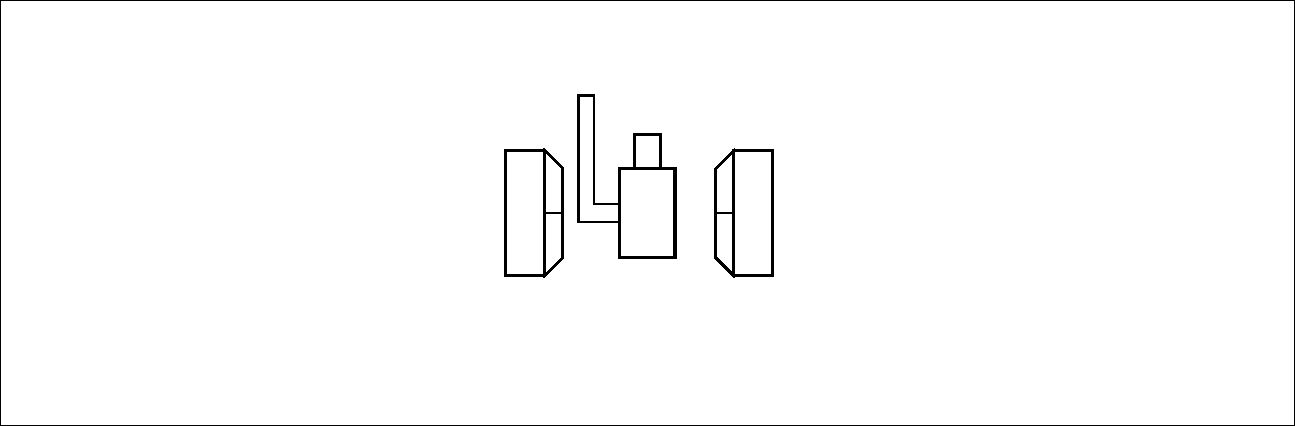
\includegraphics[width=0.9\textwidth]{./operando_epr/figures/cwEPR_spectrometer_diagram.pdf}
	\caption{Diagram of an X band cwEPR spectrometer combined with an electrochemical setup.}
	\label{fig:cwerp_spectrometer}
\end{figure}

A basic cwEPR spectrometer consists of a magnet, a microwave source, a microwave resonator and a microwave detector. Figure~\ref{fig:cwerp_spectrometer} depicts those elements with more details, including the sample - an electrochemical cell that is placed inside the microwave resonator and its state of charge controlled with an external potentiostat.

\par
Continuous microwaves are generated with a klystron (MW source in Figure~\ref{fig:cwerp_spectrometer}) and directed towards the resonator (resonating cavity) through the signal arm that contains a variable attenuator and a circulator. The circulator directs the microwaves from the source to the cavity and passes the microwaves reflected from the cavity further to the microwave detector. The adjustable coupling iris between the circulator and the resonating cavity allows one to match the impedance of the cavity to the impedance of the signal arm so that minimal microwave power is reflected back from the cavity at a non-resonant field $B_0$. That impedance matching is called critical coupling. At the microwave detector, the microwaves reflected from the cavity are compensated by the microwaves with fixed microwave power and an adjustable phase, that pass through the reference arm. The signals from the two arms interfere destructively at the detector, so that there is no signal at the detector for non-resonant $B_0$.

\par
When the resonance condition (Eq.~\ref{eq:epr_resonance_condition}) is met, the incident microwaves are being absorbed by the sample and the resonator's $Q$ factor slightly changes. A $Q$ factor of a system defines the dissipation of energy of the system per oscillation period. $Q$ can be measured as the width of the resonance profile $\Delta\nu$ with respect to the resonance frequency $\nu_0$: $Q=\frac{\Delta\nu}{\nu_0}$. The change in the $Q$ factor due to the resonance absorption of microwaves by the sample decouples the resonator from the signal arm, that causes additional reflections in the signal arm. These additional reflected microwaves in the signal arm are not compensated by the reference arm. The uncompensated microwaves excite the microwave detector - a biased semiconductor diode that has a linearly changing conductivity in the range corresponding to the incident microwave power. The typically high $Q\gg1$ factor of the resonator further increases the SNR, as decoupling of a resonator with higher $Q$ leads to a larger reflected microwave power.

\par
To ensure that only the magnetic component of the microwave is interacting with the sample, a standing microwave is formed in the resonating cavity. In the center of the cavity, the magnetic component of the microwave is maximized and the electric component is quenched. When a small sample is inserted in the center of the cavity, it is mostly the magnetic component of the microwave that is interacting with it. That allows one to drive magnetic dipole transitions without heating up the sample by the electric component. For larger samples as, for example, working electrochemical cells, the separation between the electric and magnetic microwave components does not hold within the full sample volume. Furthermore, the insertion of a cell containing metal electrodes and polar electrolyte into a resonator changes the distribution of the microwave field in it and leads to a non-resonant microwave absorption which drastically lowers the $Q$ factor (hence SNR), and mixes the dispersion component into the microwave absorption signal, distorting the spectral shape.

\paragraph{cwEPR spectrum}
A cwEPR spectrum shown in Figure~\ref{fig:cwerp_free_electron} is microwave absorption of a sample recorded with respect to the magnetic field $B_0$. A phase sensitive detection with shallow, low-frequency modulation of $B_0$ increases the signal-to-noise ratio (SNR) of the cwEPR signal and yields the derivative of the microwave absorption profile $dA/dB_0$.



\paragraph{Line Broadening}
The microwave absorption profiles in the EPR spectra have finite widths. The spectral lines of liquid samples are broadened mostly by the dynamic effects (relaxation, tumbling, chemical exchange), while the lines of solid state samples are broadened by static effects (orientational disorder, unresolved hyperfine splittings, distributions in $\textbf{g}$, $\textbf{A}$, and $\textbf{D}$ values)~\cite{Stoll2006}.\\

According to the stochastic, gaussian random modulation theory of exchange narrowing, the width of a strongly exchange narrowed EPR line (HWHM) is given by
\begin{equation}
\label{eq:exch_narrowing}
\Delta B_0 \approx\frac{10}{3}\left(\frac{H_p^2}{H_e}\right)
\end{equation}
and the resonance lineshape is lorentzian. $H_p$ is the mean square dipolar field and $H_e$ is an effective exchange field which is proportional to the mean exchange integral $J$~\cite{Oreilly_1971}. Therefore at high spin concentrations the spectral line shape depends on both exchange and dipolar couplings between the spins.\\



\section{Fundamentals of Pulsed EPR Spectroscopy}
\label{ch:pulsed_epr}

In contrast to the continuous-wave excitation described in the previous Section~\ref{subs:cwEPR_spectroscopy}, pulsed excitation of the spin system allows for time-resolved probing and for measuring spin relaxation times that is the basics of the magnetic resonance imaging. The microwave pulses at the resonance frequency cause coherent spin motion that can be controlled through the appropriate pulse sequence. This section introduces the key concepts in pulsed EPR spectroscopy and the methods for measuring spin relaxation times.

\subsection{Bloch Equations}
The macroscopic magnetization of a sample is given as a vector sum of all its individual magnetic moments. In a paramagnetic sample exposed to a static magnetic field $\vec{B_0}=\left(0,0,B_0\right)$, electron spins align with the field and create a macroscopic magnetization $\vec{M_0}=\left(0,0,M_0\right)$ along the field direction. To derive the time evolution of the $\vec{M_0}$ one does not need to solve the Schroedinger equation, as the quantum-mechanical expectation value of any quantity follows in its time dependence exactly the classical equations of motion~\cite{Bloch_1946}. The magnetization vector $\vec{M_0}$ is an angular momentum. Any change in $\vec{M_0}$ in the magnetic field causes a torque. Any deviation of $\vec{M_0}$ from the equilibrium state $\vec{M_0}=\left(0,0,M_0\right)$ leads to a relaxation to the equilibrium state after some time. From these facts, with a generalization to time-dependent magnetic fields, follows a set of equations known as the Bloch equations:

\begin{equation}
\label{eq:Bloch}
\frac{dM_x(t)}{dt} = \gamma\left(\vec{M}(t)\times\vec{B}(t)\right)_x - \frac{M_x(t)}{T_2}
\end{equation}
\begin{equation}
\nonumber
\frac{dM_y(t)}{dt} = \gamma\left(\vec{M}(t)\times\vec{B}(t)\right)_y - \frac{M_y(t)}{T_2}
\end{equation}
\begin{equation}
\nonumber
\frac{dM_z(t)}{dt} = \gamma\left(\vec{M}(t)\times\vec{B}(t)\right)_z - \frac{M_z(t)-M_0}{T_1}
\end{equation}

$T_1$ and $T_2$ are the longitudinal and transverse relaxation times, the empirically determined parameters of the spin ensemble, that describe the spin-lattice and spin-spin interactions, respectively. A solution to Eq.~\ref{eq:Bloch} with $\vec{B_0}(t) = \left(0,0,B_0\right)$ is a precession around $z$ axis that over time spirals back to the equilibrium state $\vec{M_0}$:


\begin{equation}
\vec{M}(t)=R_z(\omega_0t)\vec{M_0}(t)e{^{-\mathscr{R}t}}
\end{equation}

Where 

\begin{equation}
R_z(\phi)=
\begin{pmatrix}
    \cos{\phi} & -\sin{\phi} & 0\\
	\sin{\phi} & \cos{\phi} & 0\\
	0 & 0 & 1
  \end{pmatrix}
\end{equation}

is the rotation matrix around the $z$ axis, 

\begin{equation}
\mathscr{R}=
\begin{pmatrix}
    \frac{1}{T_2} & 0 & 0\\
	0 & \frac{1}{T_2} & 0\\
	0 & 0 & \frac{1}{T_1}
  \end{pmatrix}
\end{equation}
is the matrix of relaxation times, $\omega_0$ is the Larmor frequency and $\gamma$ is the gyromagnetic ratio.\\


Bloch showed that a microwave field $\vec{B}_1(t)$ at right angles to $\vec{B_0}$ causes a forced precession of $\vec{M}$ around the $\vec{B_0}$ with decreasing latitude (nutation), as the Larmor frequency
approaches the frequency of the microwave field. Thus, resonant $\vec{B_1}$ results a component of $\vec{M}$ at right angles to both $\vec{B}_0$ and $\vec{B}_1$ that lies in the $xy$ plane and can induce observable voltages~\cite{Bloch_1946}. A microwave pulse of amplitude $B_1^0$ and length $\tau$, $B_1(t,\tau) = B_1^0\cos(\omega t)$rect$(t,\tau)$, inclines the $\vec{M}$ towards the $xy$ plane by angle $\theta \sim B_1^0\tau$. A pulse that inclines $\vec{M}$ by $\pi/2$ and lays it into the $xy$ plane, is called a $\pi/2$ pulse. A $\pi$ pulse is defined in a similar way. The angle $\theta$ at which the pulse of a duration $t$ and intensity of $B_1$ is turning the mganetization vector is determined by the Rabi frequency $\Omega=\gamma B_1$: $\theta=\Omega t = \gamma B_1 t$. The duration of a pulse depends on the used microwave power reciprocally.


\subsection{Refocused Spin Echo}
\label{subs:spin_echo}

\begin{figure}[h]
\center
	\includegraphics[width=1\textwidth]{./epr_basics/fse.pdf}
	\caption{Top: two-pulse sequence for observing a spin echo. Bottom: time evolution of the macroscopic magnetization in the rotating frame of reference. a): magnetization at equilibrium, b): rotation of magnetization to the $xy$ plane after a $\pi/2$ pulse, c): vanishing of transverse magnetization due to spin dephasing, d): inversion of the precessing direction of spins in the $xy$ plane after the $\pi$ pulse, e): refocusing of transverse magnetization.}
	\label{fig:spin_echo_diagram}
\end{figure}


The Hahn Echo sequence shown in Figure~\ref{fig:spin_echo_diagram} consists of two pulses, the $\pi/2$ pulse and the $\pi$ pulse, separated in time by $\tau$: $\pi/2 - \tau - \pi - \tau - echo$. Initially, the macroscopic magnetization of the spin system is aligned along $\vec{B_0}$: $\vec{M}_0=M_Z~\vec{e_Z}$ (Figure~\ref{fig:spin_echo_diagram}~a). During the $\pi/2$ microwave pulse, $\vec{M}$ nutates to the $xy$ plane (Figure~\ref{fig:spin_echo_diagram}~b), where it keeps precessing about $\vec{e_Z}$ after the end of the pulse. The difference in local environments for all spins excited by the pulse, as well as the interactions between the spins that make up $\vec{M}$, leads to slightly different precession frequencies $\omega_L^i$ of the spins (Figure~\ref{fig:spin_echo_diagram}~c). After some time $\tau$, the difference in the precession frequencies translates into the differences in phases so that the vector sum of the excited spins averages down to $\vec{0}$ for sufficiently long $\tau$ (Figure~\ref{fig:spin_echo_diagram}~d). In other words, the excited spin packet loses coherency with time.\\ 
The dephasing of the individual magnetic moments due to different local spin environments can be reversible if the individual offsets of the precession frequencies do not depend on time, as is the case for separated radicals in an inhomogeneous solid. In such case, a $\pi$ pulse can be applied to the spin system to flip every single spin in the dephased spin packet by 180$^{\circ}$ in a plane containing $\vec{e}_Z$ (Figure~\ref{fig:spin_echo_diagram}~e), so that the spins keep precessing in the $xy$ plane, but the direction of precession is now inverted for them, leading to refocusing - the effect that is opposite to the initial dephasing. So a $\tau$ after the $\pi$ pulse excites the spin packet, the accumulated phase differences become the smallest and the packet recovers its macroscopic magnetization $\vec{M}$ that oscillates in the $xy$ plane with $\langle\omega_L^i\rangle$ and can be detected. The recovered $\vec{M}$ at $t=\tau$ after the $\pi$ pulse is called the refocused spin echo (Figure~\ref{fig:spin_echo_diagram}~f). The difference in $\omega_L^i$ leads to a further dephasing of the considered spin packet and to the vanishing of $\vec{M}$.\\


\subsection{Spin Relaxation Times}
There are two decay constants in Eq.~\ref{eq:Bloch}, $T_1$ and $T_2$. $T_1$ is the longitudinal relaxation time that defines the decay of the $M_Z$ component back to the equilibrium state along the $B_0$ axis ($M_Z = +M_0$). The longitudinal spin relaxation in solids in the presence of magnetic fields happens through scattering to the lattice phonons~\cite{Lunghi2019}, so $T_1$ is traditionally called the spin-lattice relaxation time. The transverse relaxation time $T_2\leq T_1$ is the decay constant of the transverse components $M_Y$ and $M_Z$ due to the inter-spin interactions that cause irreversible spin dephasing that cannot be reverted with a $\pi$ pulse described in the subsection above (\ref{subs:spin_echo}). $T_2$ is, therefore, a measure of spin concentration. Instead of $T_2$, an important experimentally observable value is the phase memory time $T_m$, which is the decay constant of the transverse magnetization caused by the combination of spin dephasing and other irreversible effects such as instantaneous diffusion~\cite{Schweiger2001,Daniel2022} caused by the broad-band microwave pulses ($T_{ID}$):

\begin{equation}
\label{eq:Tm}
\frac{1}{T_m} = \frac{1}{T_2} + \frac{1}{T_{ID}}
\end{equation} 


\subsection{Pulsed EPR Instrumentation}
The most simple pulsed EPR experiment is the detection of the refocused spin echo described in Section~\ref{subs:spin_echo}. To perform a pulsed EPR experiment, an EPR spectrometer is equipped with a pulse generator that is show on the left in Figure~\ref{fig:pepr_spectrometer_diagram}. The refocused spin echo can is observed within the spin relaxation time, so short microwave pulses have to be used. The short spin relaxation times dictate the length of the pulse sequence and require one to use shorter pulses. That requires a high power of the microwave pulse to realize the two-pulse sequence described in Section~\ref{subs:spin_echo}. For a $\pi$ pulse as long as $t_{\pi}=100$~ns one requires $B_1=\frac{\pi}{\gamma t}\approx1.1$~mT which translates to a microwave power density of $P_A=\vec{E_1}\times\vec{H_1}=\frac{c{B_1}^2}{\mu_0}\approx10^8$~W/m. For a sample with area $A=5~$mm$^2$ the required microwave power is in the range of kW so the microwave pulses are amplified with a traveling wave tube (TWT) amplifier. The resonating cavity with $Q\approx100$ is used to enhance the power density of the generated microwaves and to separate spatially their magnetic and electric components.

\begin{figure}[h]
\center
	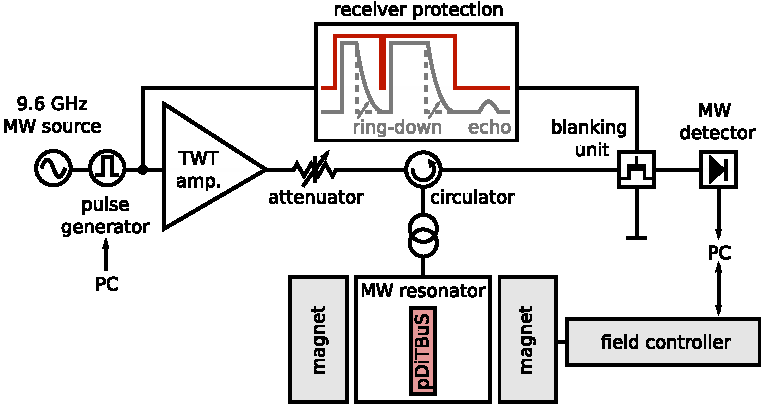
\includegraphics[width=1\textwidth]{./pulse/figures/pEPR_spectrometer_diagram.pdf}
	\caption{Diagram of a pulsed EPR spectrometer. Microwaves generated by the 9.6~GHz are modulated by the output of the pulse generator that is controlled by a PC. The modulated microwave pulses are amplified by the traveling wave tube amplifier (TWT) and directed to the resonator through a variable attenuator. The blanking unit protects the microwave detector by suppressing the high-intensity signal caused by the ring-down of the resonator. The blanking unit is controlled by the receiver protection circuit that is triggered by the pulse sequence.}
	\label{fig:pepr_spectrometer_diagram}
\end{figure}

In contrast to the high-power microwave excitation, the spin echo signal is typically in the range of nW. A protection circuit is used to blank the nW-sensitive microwave receiver from the excitation pulse that is 12 orders of magnitude beyond the receivers's range. The protection circuit shown in Figure~\ref{fig:pepr_spectrometer_diagram} consists of a blanking unit and a protection pulse generator that is synchronized with the microwave pulse sequence. The duration of the protection pulse is longer than the microwave pulse, because of the finite pulse responce of the resonating cavity. The finite pulse responce of the cavity, or ``ring-down'', postpones the time at which the spin echo can be detected -- this becomes critical in systems with short spin relaxation times.

\subsection{Pulse Sequences and Measurement Techniques}
\subsubsection{Echo-Detected Field Sweep}
The tho-pulse Hahn echo sequence shown in Section~\ref{subs:spin_echo} results in a spin echo only when the static magnetic field $B_0$ is resonant to the excited spins. When a sample spins have anisotropic $A$ and $g$ values and/or different molecular environments, the different intensities of the spin echo will be detected at different $B_0$. Recording the spin echo with linearly changing $B_0$ is called the echo-detected field sweep (EDFS). Observing cwEPR requires short spin relaxation to avoid saturation of continuous microwaves. In contrast, the EDFS signals comes from the species with longer relaxation times. The faster relaxing species, as, for example, densely packed nitroxide radicals in a discharged cathode of an ORB, produce no EDFS signal, as their spin echo decays within the receiver protection pulse.

\subsubsection{Spin Echo Decay and Phase Memory Time}
The measurement of transverse spin relaxation time $T_2$ can be done follows: The intensity of the spin echo is recorded as a function of the delay time $\tau$ between the $\pi/2$ and the $\pi$ pulse of the two-pulse sequence (see Figure~\ref{fig:Tm_diagram}). The decay of the amplitude of the spin echo as a function of $\tau$ is the result of irreversible spin dephasing that is described by an exponential decay with the time constant $T_m$ - the phase memory time. Knowing the individual contributions to the $T_m$ one can estimate $T_2$ by using Eq.~\ref{eq:Tm}.

\begin{figure}[h]
\center
	
\includegraphics[width=1\textwidth]{./epr_basics/echo_decay.pdf}
	\caption{Two-pulse sequence with variable delay for observing a decay of the spin echo and determining the phase memory time $t_m$.}
	\label{fig:Tm_diagram}
\end{figure}

\subsubsection{Inversion Recovery and Spin-Lattice Relaxation Time}
The longitudinal spin relaxation time $T_1$ can be measured in an inversion recovery experiment. The three-pulse sequence shown in Figure~\ref{fig:T1_diagram}~a) is the inversion recovery sequence. In the inversion recovery experiment, three microwave pulses with various spacing between the first and the second pulse are used to measure the time that the longitudinal ($M_Z$) component of the magnetization vector takes to recover from $(0,0,-M_Z)$ (Figure~\ref{fig:T1_diagram})~d) to the equilibrium state $(0,0,M_Z)$ (Figure~\ref{fig:T1_diagram})~c). The magnetization vector is first flipped from $(0,0,M_Z)$ to $(0,0,-M_Z)$ by a $\pi$ pulse (Figure~\ref{fig:T1_diagram}~c-d). After a time $\tau$, some of the spins recover to $(0,0,1)$ state, reducing the magnitude of the $M_Z$ component due to the spin-lattice relaxation as shown in Figure~\ref{fig:T1_diagram}~d-e). Then a two-pulse echo sequence (Figure~\ref{fig:T1_diagram}~e-g) is applied to detect the magnitude of the remaining longitudinal magnetization. As $\tau$ is varied and the decreasing amplitude of the spin echo is recorded, one observes the longitudinal spin relaxation, or the spin-lattice relaxation time $T_1$. For short delay times $\tau$, the detected echo intensity is negative, as most of the spins remain inverted. With longer $\tau$ less spins remain in the inverted state and eventually the detected echo intensity becomes positive. The dependence of the echo intensity on $\tau$ is the inversion recovery transient that is shown in Figure~\ref{fig:T1_diagram}~b). From an exponential fit to the inversion recovery transient one obtains the spin-lattice relaxation time $T_1$.

\begin{figure}[h]
\center
	\includegraphics[width=1\textwidth]{./epr_basics/inversion_recovery.pdf}
	\caption{a): Three-pulse sequence with variable delay between the first and the second pulse for observing inversion recovery. b): typical inversion recovery transient. The longitudinal relaxation time $T_1$ is the fit parameter. c): inversion of the magnetization by the initial $\pi$ pulse. b): recovery of the magnetization after time $\tau$ due to the spin-lattice relaxation. e): rotation of the remaining magnetization to the $xy$ plane with a $\pi/2$ pulse. f),g) - refocusing the magnetization in the $xy$ plane to detect the remaining magnetization with a spin echo.}
	\label{fig:T1_diagram}
\end{figure}
